%% AC5211 Multimedia Database -- final-project poster (A0 portrait, 2 columns).
%% Condensed from ../final-report/main.pdf. Plan: PLAN.md.
%% Build:  latexmk -pdf poster.tex      (pdfLaTeX)
%% Every number from our own runs comes from ../final-report/generated/numbers.tex
%% and ../final-report/generated/curve_*.csv; IRRA numbers are quoted from [1].

\documentclass[25pt, a0paper, portrait, margin=15mm, innermargin=12mm,
    blockverticalspace=12mm, colspace=16mm, subcolspace=0mm]{tikzposter}

\usepackage[utf8]{inputenc}
\usepackage[T1]{fontenc}
\usepackage{tgheros}
\renewcommand{\familydefault}{\sfdefault}
\usepackage{amsmath, amssymb}
\usepackage{booktabs}
\usepackage{array}
\usepackage{enumitem}
\usepackage{pgfplots}
\pgfplotsset{compat=1.18, every axis/.append style={/pgf/number format/assume math mode=true}}
\usetikzlibrary{positioning,arrows.meta,calc,shapes.geometric}
\usepackage{qrcode}

% AUTO-GENERATED by scripts/gen_results.py -- do not edit by hand.
\newcommand{\sdmPeakEp}{9}
\newcommand{\sdmPeakR}{58.85}
\newcommand{\sdmPeakRfive}{80.30}
\newcommand{\sdmPeakRten}{89.15}
\newcommand{\sdmPeakM}{45.46}
\newcommand{\sdmPeakMINP}{23.29}
\newcommand{\sdmBestM}{45.56}
\newcommand{\sdmBestMEp}{14}
\newcommand{\sdmConvR}{57.18}
\newcommand{\sdmConvRsd}{0.28}
\newcommand{\sdmConvM}{45.42}
\newcommand{\sdmConvMsd}{0.13}
\newcommand{\sdmEpochs}{20}
\newcommand{\sdmLastR}{56.95}
\newcommand{\sdmDrop}{1.90}
\newcommand{\sdmLossFirst}{21.16}
\newcommand{\sdmLossLast}{8.07}
\newcommand{\sdmEpNineR}{58.85}
\newcommand{\sdmEpFourR}{55.50}
\newcommand{\sdmEpThreeR}{52.55}
\newcommand{\sdmMinPerEp}{7.2}
\newcommand{\mpcePeakEp}{3}
\newcommand{\mpcePeakR}{55.70}
\newcommand{\mpcePeakRfive}{76.40}
\newcommand{\mpcePeakRten}{85.50}
\newcommand{\mpcePeakM}{42.35}
\newcommand{\mpcePeakMINP}{20.78}
\newcommand{\mpceBestM}{42.92}
\newcommand{\mpceBestMEp}{5}
\newcommand{\mpceConvR}{48.85}
\newcommand{\mpceConvRsd}{0.15}
\newcommand{\mpceConvM}{40.82}
\newcommand{\mpceConvMsd}{0.06}
\newcommand{\mpceEpochs}{30}
\newcommand{\mpceLastR}{49.00}
\newcommand{\mpceDrop}{6.70}
\newcommand{\mpceLossFirst}{4.26}
\newcommand{\mpceLossLast}{0.61}
\newcommand{\mpceEpNineR}{51.05}
\newcommand{\mpceEpFourR}{53.65}
\newcommand{\mpceEpThreeR}{55.70}
\newcommand{\mpceMinPerEp}{6.9}
\newcommand{\ncePeakEp}{3}
\newcommand{\ncePeakR}{55.20}
\newcommand{\ncePeakRfive}{76.65}
\newcommand{\ncePeakRten}{85.25}
\newcommand{\ncePeakM}{42.15}
\newcommand{\ncePeakMINP}{20.64}
\newcommand{\nceBestM}{43.07}
\newcommand{\nceBestMEp}{6}
\newcommand{\nceConvR}{48.52}
\newcommand{\nceConvRsd}{0.25}
\newcommand{\nceConvM}{40.56}
\newcommand{\nceConvMsd}{0.14}
\newcommand{\nceEpochs}{27}
\newcommand{\nceLastR}{48.60}
\newcommand{\nceDrop}{6.60}
\newcommand{\nceLossFirst}{2.10}
\newcommand{\nceLossLast}{0.29}
\newcommand{\nceEpNineR}{51.75}
\newcommand{\nceEpFourR}{53.80}
\newcommand{\nceEpThreeR}{55.20}
\newcommand{\nceMinPerEp}{6.6}
\newcommand{\gapSdmNceR}{3.65}
\newcommand{\gapSdmNceM}{3.31}
\newcommand{\gapSdmMpceR}{3.15}
\newcommand{\gapSdmMpceM}{3.11}
\newcommand{\gapSdmMpceBestM}{2.64}
\newcommand{\mpNceDiffR}{0.18}
\newcommand{\mpNceDiffRsd}{0.59}
\newcommand{\mpNceDiffRmax}{1.45}
\newcommand{\mpNceDiffM}{0.17}
\newcommand{\mpNceDiffMmax}{0.64}
\newcommand{\lossRatioLo}{2.03}
\newcommand{\lossRatioHi}{2.12}
\newcommand{\nPairedEp}{27}
\newcommand{\sdmLrFour}{9.92}
\newcommand{\sdmLrNine}{7.26}
\newcommand{\nceLrFour}{9.97}
\newcommand{\nceLrNine}{8.84}
\newcommand{\lrMaxRelDiff}{18}
\newcommand{\gapIrraR}{1.35}
\newcommand{\gapIrraM}{1.71}
\newcommand{\gapIrraSdmR}{1.65}
\newcommand{\gainIrraSdm}{3.15}
\newcommand{\nTrainable}{491\,520}
\newcommand{\nTotal}{150\,109\,185}
\newcommand{\nTotalM}{150.1}
\newcommand{\nBackbone}{149\,617\,665}
\newcommand{\nBackboneM}{149.6}
\newcommand{\trainPct}{0.33}
\newcommand{\nLoraModules}{96}
\newcommand{\ckptMiB}{1.88}
\newcommand{\fullMiB}{571}
\newcommand{\sizeRatio}{304}
\newcommand{\idHeadM}{1.90}
\newcommand{\batchSize}{64}
\newcommand{\sdmRounds}{20}
\newcommand{\nceRounds}{30}
\newcommand{\mpceRounds}{30}
\newcommand{\posFrac}{1.52}
\newcommand{\oneHotFrac}{98.48}
\newcommand{\nExamples}{37\,010}
\newcommand{\logInvEps}{18.42}
\newcommand{\kClients}{15}
\newcommand{\rRounds}{30}
\newcommand{\upLoraRoundMiB}{28.1}
\newcommand{\upFullRoundGiB}{8.4}
\newcommand{\upLoraTotalGiB}{0.82}
\newcommand{\upFullTotalGiB}{251}
\newcommand{\optLoraMiB}{3.75}
\newcommand{\optFullGiB}{1.11}
\newcommand{\roundVsOneFull}{20}


% ---------------- colours: black/grey + one accent; series colours as in the report
\definecolor{ieee}{HTML}{00629B}
\definecolor{cSDM}{HTML}{2A78D6}
\definecolor{cMPCE}{HTML}{EB6834}
\definecolor{cNCE}{HTML}{1BAF7A}
\definecolor{cOurs}{HTML}{2A78D6}
\definecolor{cIRRA}{HTML}{6B6B6B}
\DeclareMathOperator{\KL}{KL}

% ---------------- minimal title and block styles
\definetitlestyle{PlainTitle}{
    width=\textwidth, roundedcorners=0, linewidth=0pt, innersep=8mm,
    titletotopverticalspace=6mm, titletoblockverticalspace=12mm,
    titlegraphictotitledistance=0pt, titletextscale=1
}{
    \draw[draw=ieee, line width=3mm]
        (\titleposleft,\titleposbottom) -- (\titleposright,\titleposbottom);
}
\defineblockstyle{PlainBlock}{
    titlewidthscale=1, bodywidthscale=1, titleleft,
    titleoffsetx=0pt, titleoffsety=0pt, bodyoffsetx=0pt, bodyoffsety=0pt,
    bodyverticalshift=0pt, roundedcorners=0, linewidth=1.5pt,
    titleinnersep=8mm, bodyinnersep=10mm
}{
    \ifBlockHasTitle
        \draw[draw=black!30, line width=\blocklinewidth]
            (blockbody.south west) rectangle (blocktitle.north east);
        \draw[draw=ieee, line width=2mm]
            (blocktitle.south west) -- (blocktitle.south east);
    \else
        \draw[draw=black!30, line width=\blocklinewidth]
            (blockbody.south west) rectangle (blockbody.north east);
    \fi
}
\usetheme{Default}
\usetitlestyle{PlainTitle}
\useblockstyle{PlainBlock}
\colorlet{backgroundcolor}{white}
\colorlet{framecolor}{white}
\colorlet{titlebgcolor}{white}
\colorlet{titlefgcolor}{black}
\colorlet{blocktitlebgcolor}{white}
\colorlet{blocktitlefgcolor}{ieee}
\colorlet{blockbodybgcolor}{white}
\colorlet{blockbodyfgcolor}{black}
\tikzposterlatexaffectionproofoff

% block with a 52 pt title and a 30 pt body
\newcommand{\pblock}[2]{\block{\huge\bfseries #1}{\large #2}}
% captions under figures: 25 pt grey
\newcommand{\pcap}[1]{\par\vspace{-0.3em}{\normalsize\color{black!65}#1\par}}
% series markers for text and tables (same shapes as in the plots)
\newcommand{\mk}[2]{\tikz[baseline=-0.6ex]\node[#1,fill=#2,draw=#2,inner sep=0pt,minimum size=0.55em]{};}
\newcommand{\mkSDM}{\mk{circle}{cSDM}}
\newcommand{\mkMPCE}{\mk{regular polygon,regular polygon sides=3,minimum size=0.75em}{cMPCE}}
\newcommand{\mkNCE}{\mk{rectangle}{cNCE}}
% big number + label (block 4)
\newcommand{\stat}[3][0.32]{\begin{minipage}[t]{#1\linewidth}\centering
    {\Huge\bfseries #2}\\[0.1em]{\normalsize #3}\end{minipage}}
\setlist{leftmargin=1.1em, itemsep=0.3em, topsep=0.3em}
\renewcommand{\cite}[1]{[#1]}

% ---------------- header
\title{LoRA Meets Similarity Distribution Matching: Parameter-Efficient CLIP Tuning for Text-Based Person Search}
\author{Do Thanh Tung \quad{\color{black!60}$\cdot$}\quad Student ID 20252432M}
\institute{AC5211 Multimedia Database --- Final Project \quad{\color{black!60}$\cdot$}\quad Hanoi, Vietnam}
\makeatletter
\settitle{%
  \begin{minipage}[c]{0.85\linewidth}\raggedright
    {\fontsize{80}{96}\selectfont\bfseries LoRA Meets Similarity Distribution Matching:\\
     Parameter-Efficient CLIP Tuning\\ for Text-Based Person Search\par}\vspace{0.6em}
    {\huge \@author\par}\vspace{0.3em}
    {\LARGE\color{black!65}\@institute\par}
  \end{minipage}\hfill
  \begin{minipage}[c]{0.13\linewidth}\centering
    \qrcode[height=10cm]{https://github.com/thanhtungdo2211/master-thesis}\par\vspace{0.3em}
    {\normalsize\color{black!65} code on GitHub}
  \end{minipage}}
\makeatother

\begin{document}
\maketitle

\begin{columns}
% =====================================================================
\column{0.5}

\pblock{1\quad Motivation \& Questions}{
Text-based person search ranks a gallery of pedestrian images by a free-form
description. IRRA~\cite{1} fine-tunes all \nBackboneM\,M parameters of
CLIP~\cite{2}. In federated learning every client uploads the trainable part
in every round, so its size sets the communication cost. We ask two questions:
\begin{itemize}
  \item How much accuracy does a \emph{frozen} CLIP with LoRA~\cite{3}
        and the SDM loss alone give up, and how much does it save?
  \item Why does SDM beat InfoNCE? IRRA credits several positives
        per batch. We test this.
\end{itemize}
\vspace{0.4em}
{\normalsize
\setlength{\tabcolsep}{0pt}\renewcommand{\arraystretch}{1.15}
\begin{tabular}{@{}>{\raggedright\arraybackslash}p{0.44\linewidth}@{\hspace{0.04\linewidth}}>{\raggedright\arraybackslash}p{0.52\linewidth}@{}}
  \textbf{\color{black!70}Existing (prior work)} & \textbf{\color{ieee}Ours} \\[0.1em]
  \hline\noalign{\vspace{0.3em}}
  CLIP ViT-B/16~\cite{2}; LoRA~\cite{3}       & Frozen CLIP + rank-4 LoRA on both encoders \\
  SDM loss; IRRA results on RSTPReid~\cite{1,4} & SDM as the \emph{only} loss; all LoRA runs \\
  MAE robustness~\cite{5}                     & One-hot analysis of SDM; MPCE control; loss ablation \\
\end{tabular}}
}

\pblock{2\quad Method: LoRA-tuned CLIP, SDM only}{
\begin{center}
\resizebox{0.92\linewidth}{!}{% Pipeline figure, shared by the report (sections/04_method.tex) and the poster.
% Needs: TikZ libraries positioning, arrows.meta, calc; colour cOurs.
% Sizes are absolute (mm), so the font is fixed at 7 pt; the poster scales the whole picture.
% Grid-aligned: both encoder lanes have identical widths, all arrows are horizontal or vertical.
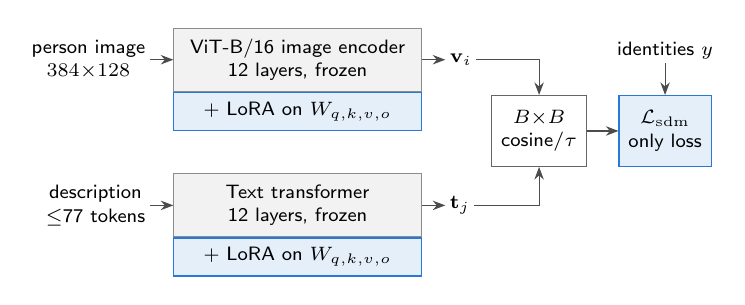
\begin{tikzpicture}[
  font=\fontsize{7}{8.5}\selectfont,
  enc/.style={draw=black!45, fill=black!5, text width=29mm, align=center,
              inner sep=1.2mm, minimum height=8mm},
  lora/.style={draw=cOurs, fill=cOurs!12, text width=29mm, align=center,
               inner sep=1.2mm, minimum height=4.5mm},
  op/.style={draw=black!60, fill=white, align=center, inner sep=1.2mm, minimum height=9mm},
  loss/.style={draw=cOurs, fill=cOurs!12, align=center, inner sep=1.2mm, minimum height=9mm},
  io/.style={align=center, inner sep=0.5mm},
  arr/.style={-{Stealth[length=1.6mm]}, draw=black!70}]
% ---- image lane (top) and text lane (bottom), same x positions
\node[enc]  (vit) at (0, 7.5mm)  {ViT-B/16 image encoder\\12 layers, frozen};
\node[lora, below=0pt of vit]     (lv)  {+ LoRA on $W_{q,k,v,o}$};
\node[enc]  (tr)  at (0,-11mm)   {Text transformer\\12 layers, frozen};
\node[lora, below=0pt of tr]      (lt)  {+ LoRA on $W_{q,k,v,o}$};
\node[io, left=3mm of vit] (img) {person image\\$384{\times}128$};
\node[io, left=3mm of tr]  (txt) {description\\$\le$77 tokens};
\node[io, right=3mm of vit] (v) {$\mathbf{v}_i$};
\node[io, right=3mm of tr]  (t) {$\mathbf{t}_j$};
% ---- similarity and loss, centred between the two lanes
\path (v) -- (t) coordinate[pos=0.5] (mid);
\node[op]   (S) at ($(mid)+(10mm,0)$) {$B{\times}B$\\cosine$/\tau$};
\node[loss, right=4mm of S] (L) {$\mathcal{L}_{\mathrm{sdm}}$\\only loss};
\node[io, above=4mm of L] (y) {identities $y$};
% ---- arrows (orthogonal only)
\draw[arr] (img) -- (vit);
\draw[arr] (txt) -- (tr);
\draw[arr] (vit) -- (v);
\draw[arr] (tr)  -- (t);
\draw[arr] (v) -| (S.north);
\draw[arr] (t) -| (S.south);
\draw[arr] (S) -- (L);
\draw[arr] (y) -- (L);
\end{tikzpicture}
}
\end{center}
\pcap{Grey: frozen CLIP. Blue: the only trainable parameters.}
\vspace{0.4em}
Each attention projection becomes
$W'\mathbf{x} = W\mathbf{x} + \tfrac{\alpha}{r}BA\,\mathbf{x}$ ($r=4$, $\alpha=8$):
\nLoraModules{} modules, \nTrainable{} trainable parameters (\trainPct\%).
No ID classifier, no IRR encoder. $BA$ merges into $W$ after training,
so inference costs the same as CLIP.
}

\pblock{3\quad Analysis: what SDM really optimises}{
\textbf{Step 1: a second positive is rare.} IRRA motivates SDM with batches holding
several examples of one person. RSTPReid has 10 per person among \nExamples, so in a
random batch of \batchSize{} only \textbf{\posFrac\%} of rows have a second one:
in \oneHotFrac\% of rows SDM's target is one-hot, as in InfoNCE.

\vspace{0.4em}
\textbf{Step 2: the loss is still different.} With a one-hot target, SDM becomes
\[
  \ell^{\mathrm{sdm}}_i \approx
  \underbrace{\lambda\,(1-p_{i,i})}_{\text{scaled MAE}}
  - \underbrace{H(p_{i,\cdot})}_{\text{entropy bonus}}
  \qquad\text{vs.}\qquad
  \ell^{\mathrm{nce}}_i = -\log p_{i,i},
\]
with $\lambda=\log(1/\epsilon)=\logInvEps$. MAE is bounded and robust to label noise~\cite{5}.

\vspace{0.4em}
\textbf{Step 3: so the two losses train on different pairs.}
\begin{center}
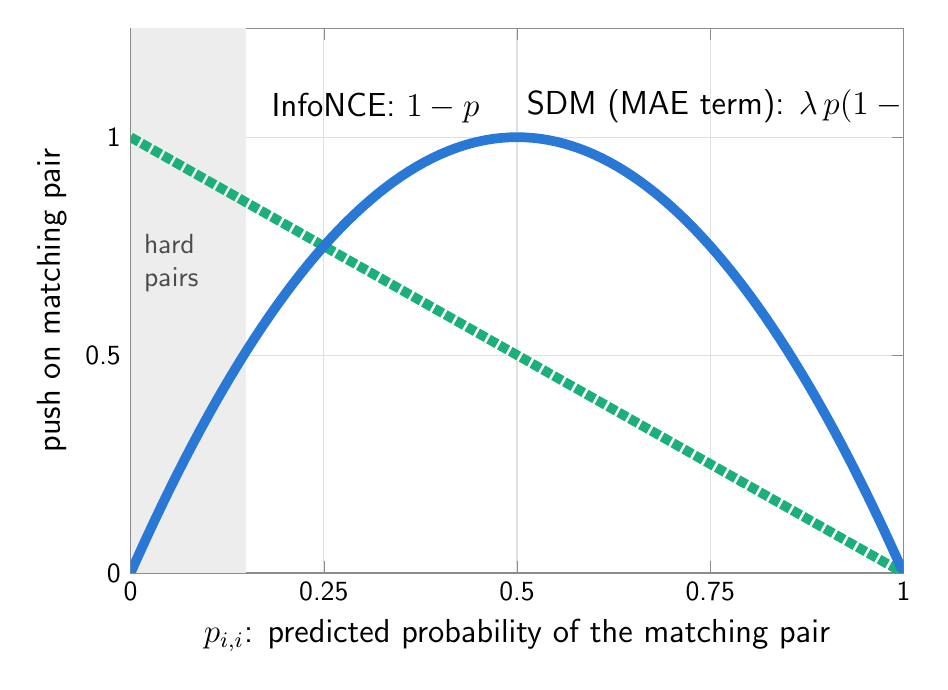
\begin{tikzpicture}
\begin{axis}[
  width=0.94\linewidth, height=8.5cm,
  xmin=0, xmax=1, ymin=0, ymax=1.25,
  xlabel={$p_{i,i}$: predicted probability of the matching pair},
  ylabel={push on matching pair},
  ytick={0,0.5,1}, xtick={0,0.25,0.5,0.75,1},
  tick label style={font=\normalsize}, label style={font=\large},
  axis line style={black!45}, tick style={black!45},
  grid=major, grid style={black!12}]
  \fill[black!7] (axis cs:0,0) rectangle (axis cs:0.15,1.25);
  \node[anchor=north west,align=left,font=\normalsize,text=black!70]
     at (axis cs:0.005,0.80) {hard\\pairs};
  \addplot[cNCE, line width=3.5pt, densely dotted, domain=0:1, samples=101] {1-x};
  \addplot[cSDM, line width=3.5pt, domain=0:1, samples=101] {4*x*(1-x)};
  \node[anchor=south west,font=\large] at (axis cs:0.17,1.01) {InfoNCE: $1-p$};
  \node[anchor=south west,font=\large] at (axis cs:0.50,1.01) {SDM (MAE term): $\lambda\,p(1-p)$};
\end{axis}
\end{tikzpicture}
\end{center}
\pcap{Analytic, each curve scaled to peak 1. InfoNCE pushes hardest on the pairs it
ranks worst, often ambiguous ones; SDM nearly ignores them.}
\vspace{0.4em}
\textbf{Test:} MPCE keeps SDM's targets but uses InfoNCE's direction, $\KL(q\Vert p)$.
If Step 3 is the reason, MPCE should behave like InfoNCE (block 5).
}

\pblock{References}{
{\small\color{black!80}
[1] D.~Jiang, M.~Ye. Cross-modal implicit relation reasoning and aligning for text-to-image person retrieval (IRRA). CVPR 2023.\par
[2] A.~Radford \textit{et al.} Learning transferable visual models from natural language supervision (CLIP). ICML 2021.\par
[3] E.~J.~Hu \textit{et al.} LoRA: Low-rank adaptation of large language models. ICLR 2022.\par
[4] A.~Zhu \textit{et al.} DSSL: Deep surroundings-person separation learning for text-based person retrieval (RSTPReid). ACM MM 2021.\par
[5] A.~Ghosh, H.~Kumar, P.~S.~Sastry. Robust loss functions under label noise for deep neural networks. AAAI 2017.\par}
}

% =====================================================================
\column{0.5}

\pblock{4\quad LoRA vs.\ full fine-tuning}{
\begin{center}
\stat{\textcolor{ieee}{\sizeRatio$\times$}}{fewer trainable params}\hfill
\stat[0.34]{0.49\,M}{trained vs.\ \nBackboneM\,M}\hfill
\stat{\ckptMiB\,MiB}{update vs.\ \fullMiB\,MiB}
\end{center}
\vspace{-0.3em}
\begin{center}
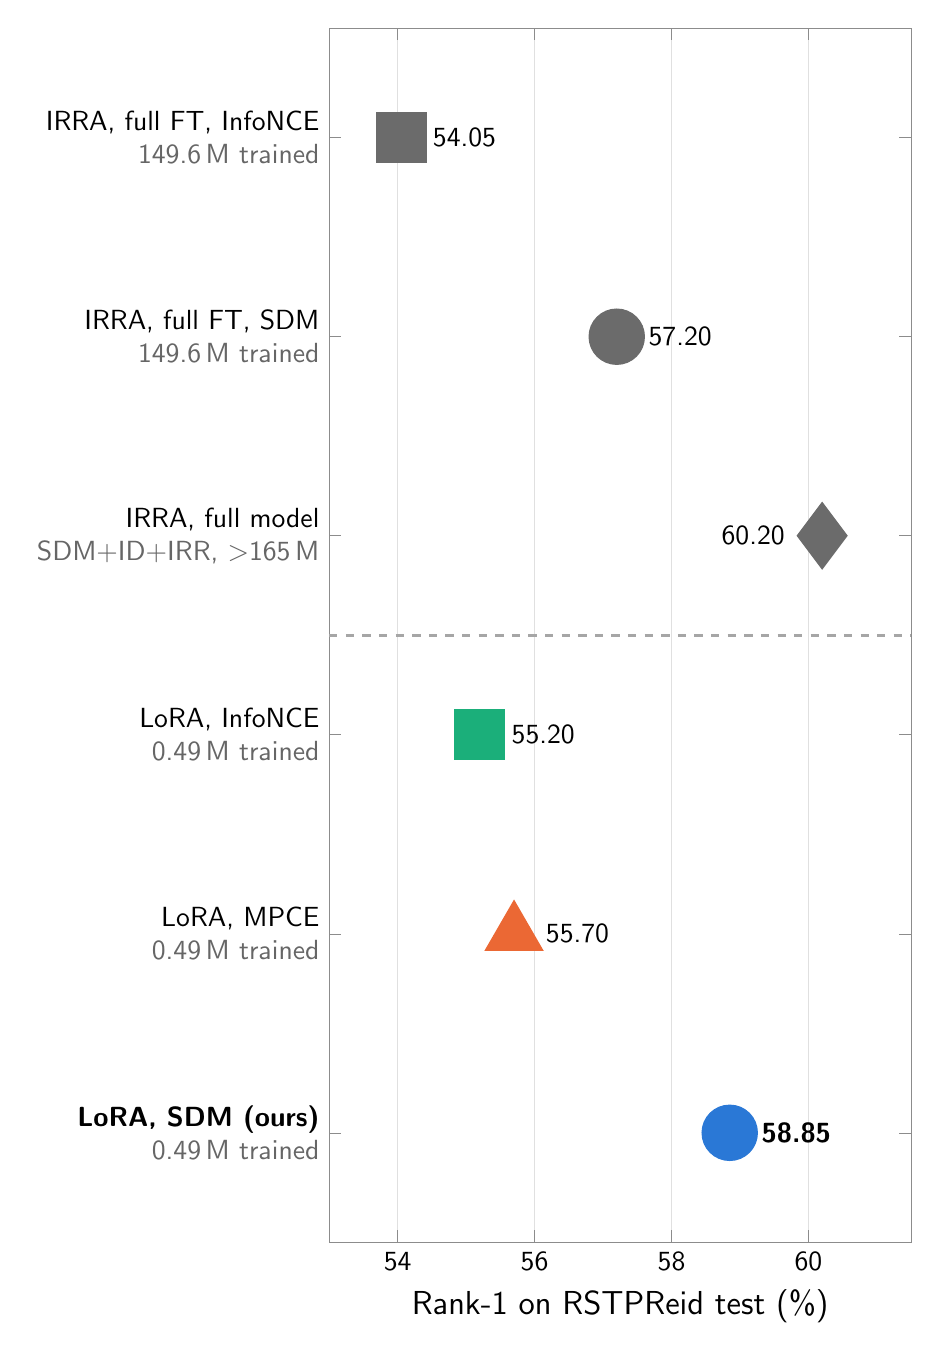
\begin{tikzpicture}
\begin{axis}[
  width=0.74\linewidth, height=17cm,
  xmin=53, xmax=61.5, ymin=0.45, ymax=6.55, y dir=reverse,
  ytick={1,...,6},
  yticklabels={
    {IRRA, full FT, InfoNCE\\\color{black!60}149.6\,M trained},
    {IRRA, full FT, SDM\\\color{black!60}149.6\,M trained},
    {IRRA, full model\\\color{black!60}SDM+ID+IRR, $>$165\,M},
    {LoRA, InfoNCE\\\color{black!60}0.49\,M trained},
    {LoRA, MPCE\\\color{black!60}0.49\,M trained},
    {\textbf{LoRA, SDM (ours)}\\\color{black!60}0.49\,M trained}},
  yticklabel style={align=right, font=\normalsize},
  xlabel={Rank-1 on RSTPReid test (\%)}, label style={font=\large},
  xtick={54,56,58,60}, tick label style={font=\normalsize},
  xmajorgrids, grid style={black!12},
  axis line style={black!45}, tick style={black!45}, clip=false]
  \draw[black!35, dashed, line width=1pt] (axis cs:53,3.5) -- (axis cs:61.5,3.5);
  % IRRA, quoted from [1]
  \addplot[only marks, mark=square*, mark size=9pt, color=cIRRA] coordinates {(54.05,1)};
  \addplot[only marks, mark=*, mark size=10pt, color=cIRRA] coordinates {(57.20,2)};
  \addplot[only marks, mark=diamond*, mark size=12pt, color=cIRRA] coordinates {(60.20,3)};
  % ours (peak epoch)
  \addplot[only marks, mark=square*, mark size=9pt, color=cNCE] coordinates {(\ncePeakR,4)};
  \addplot[only marks, mark=triangle*, mark size=12pt, color=cMPCE] coordinates {(\mpcePeakR,5)};
  \addplot[only marks, mark=*, mark size=10pt, color=cSDM] coordinates {(\sdmPeakR,6)};
  \node[right=8pt, font=\normalsize] at (axis cs:54.05,1) {54.05};
  \node[right=8pt, font=\normalsize] at (axis cs:57.20,2) {57.20};
  \node[left=10pt, font=\normalsize]  at (axis cs:60.20,3) {60.20};
  \node[right=8pt, font=\normalsize] at (axis cs:\ncePeakR,4) {\ncePeakR};
  \node[right=8pt, font=\normalsize] at (axis cs:\mpcePeakR,5) {\mpcePeakR};
  \node[right=8pt, font=\normalsize\bfseries] at (axis cs:\sdmPeakR,6) {\sdmPeakR};
\end{axis}
\end{tikzpicture}
\end{center}
\pcap{Peak R@1 (best test epoch, as IRRA reports). Grey: quoted from IRRA~\cite{1}.
Ours: one seed each; standard error $\approx$1.1\,pt.}
\vspace{0.4em}
LoRA+SDM is \textbf{on par} with SDM-only full fine-tuning: \sdmPeakR{} peak and
\sdmConvR\,$\pm$\,\sdmConvRsd{} converged vs.\ 57.20. The complete IRRA model adds
ID and IRR losses with their own parameters and is \gapIrraR\,pt higher.
}

\pblock{5\quad Why does SDM help?}{
{\normalsize
\setlength{\tabcolsep}{9pt}
\begin{center}
\begin{tabular}{@{}lllcc@{}}
  \toprule
  Loss & Target & Divergence & Peak R@1 & Conv.\ R@1 \\
  \midrule
  \mkNCE\ InfoNCE  & diagonal & cross-entropy  & \ncePeakR  & \nceConvR \\
  \mkMPCE\ MPCE    & identity & $\KL(q\Vert p)$ & \mpcePeakR & \mpceConvR \\
  \mkSDM\ SDM      & identity & $\KL(p\Vert q)$ & \textbf{\sdmPeakR} & \textbf{\sdmConvR} \\
  \bottomrule
\end{tabular}
\end{center}}
\vspace{-0.4em}
\begin{center}
\begin{tikzpicture}
\pgfplotsset{
  every axis/.append style={width=0.95\linewidth, height=9.5cm, xmin=0.5, xmax=30.5,
    tick label style={font=\normalsize}, label style={font=\large},
    grid=major, grid style={black!12}, axis line style={black!45}, tick style={black!45}},
  sdm/.style={cSDM, line width=3pt, mark=*, mark size=5pt},
  mpce/.style={cMPCE, line width=3pt, dashed, mark=triangle*, mark size=6.5pt, mark options={solid}},
  nce/.style={cNCE, line width=3pt, densely dotted, mark=square*, mark size=4.5pt, mark options={solid}}}
\begin{axis}[name=top, ylabel={R@1 (\%)}, ymin=40, ymax=61, ytick={40,45,50,55,60}, xtick={1,5,10,15,20,25,30}, xticklabels={}]
  \addplot[sdm]  table[x=epoch,y=r1,col sep=comma]{../final-report/generated/curve_sdm.csv};
  \addplot[mpce] table[x=epoch,y=r1,col sep=comma]{../final-report/generated/curve_mpce.csv};
  \addplot[nce]  table[x=epoch,y=r1,col sep=comma]{../final-report/generated/curve_nce.csv};
  \draw[cIRRA, line width=1.2pt, dashdotted] (axis cs:0.5,57.20) -- (axis cs:30.5,57.20);
  \draw[cIRRA, line width=1.2pt, dashdotted] (axis cs:0.5,54.05) -- (axis cs:30.5,54.05);
  \node[anchor=south east, font=\small, text=black!70, inner sep=3pt] at (axis cs:30.4,57.20) {IRRA full FT, SDM};
  \node[anchor=south east, font=\small, text=black!70, inner sep=3pt] at (axis cs:30.4,54.05) {IRRA full FT, InfoNCE};
\end{axis}
\begin{axis}[at={(top.south)}, anchor=north, yshift=-5mm, xlabel={epoch}, xtick={1,5,10,15,20,25,30},
  ylabel={mAP (\%)}, ymin=30, ymax=47, ytick={30,35,40,45},
  legend style={font=\normalsize, at={(0.99,0.05)}, anchor=south east,
    draw=black!30, fill=white, legend columns=3, /tikz/every even column/.append style={column sep=6mm}}]
  \addplot[sdm]  table[x=epoch,y=map,col sep=comma]{../final-report/generated/curve_sdm.csv};
  \addplot[mpce] table[x=epoch,y=map,col sep=comma]{../final-report/generated/curve_mpce.csv};
  \addplot[nce]  table[x=epoch,y=map,col sep=comma]{../final-report/generated/curve_nce.csv};
  \legend{SDM, MPCE, InfoNCE}
\end{axis}
\end{tikzpicture}
\end{center}
\vspace{-0.3em}
\begin{itemize}
  \item \textbf{Targets: no effect.} MPCE vs.\ InfoNCE changes only the target;
        R@1 differs by \mpNceDiffR\,$\pm$\,\mpNceDiffRsd\,pt on average, within noise.
  \item \textbf{KL direction: the whole gain.} SDM vs.\ MPCE changes only the direction:
        \textbf{+\gapSdmMpceR} R@1, +\gapSdmMpceM{} mAP. InfoNCE and MPCE peak at
        epoch 3, then lose \nceDrop{} and \mpceDrop\,pt; SDM improves until epoch \sdmPeakEp.
\end{itemize}
}

\pblock{6\quad Takeaways}{
\begin{center}
\fcolorbox{ieee}{white}{\parbox{0.95\linewidth}{\centering\vspace{0.3em}
  {\LARGE\bfseries\color{ieee} SDM's gain comes from the KL direction,\\
  not from multiple positives.}\vspace{0.3em}}}
\end{center}
\begin{itemize}
  \item \textbf{Efficiency:} \trainPct\% of the parameters, same R@1 as SDM-only full fine-tuning.
  \item \textbf{Why SDM helps:} it acts as a bounded MAE loss plus an entropy bonus,
        which resists overfitting on a small dataset.
  \item \textbf{Federated outlook:} with \kClients{} clients, a round uploads
        \upLoraRoundMiB\,MiB instead of \upFullRoundGiB\,GiB, and SDM has no
        identity-tied parameters to federate.
\end{itemize}
\pcap{Limitations: one seed per run; IRRA numbers are quoted, not reproduced.}
}

\end{columns}
\end{document}
